\documentclass{extbook}[14pt]
\usepackage{multicol, enumerate, enumitem, hyperref, color, soul, setspace, parskip, fancyhdr, amssymb, amsthm, amsmath, bbm, latexsym, units, mathtools}
\everymath{\displaystyle}
\usepackage[headsep=0.5cm,headheight=0cm, left=1 in,right= 1 in,top= 1 in,bottom= 1 in]{geometry}
\usepackage{dashrule}  % Package to use the command below to create lines between items
\newcommand{\litem}[1]{\item #1

\rule{\textwidth}{0.4pt}}
\pagestyle{fancy}
\lhead{}
\chead{Answer Key for Makeup Progress Quiz 1 Version B}
\rhead{}
\lfoot{6018-3080}
\cfoot{}
\rfoot{Spring 2021}
\begin{document}
\textbf{This key should allow you to understand why you choose the option you did (beyond just getting a question right or wrong). \href{https://xronos.clas.ufl.edu/mac1105spring2020/courseDescriptionAndMisc/Exams/LearningFromResults}{More instructions on how to use this key can be found here}.}

\textbf{If you have a suggestion to make the keys better, \href{https://forms.gle/CZkbZmPbC9XALEE88}{please fill out the short survey here}.}

\textit{Note: This key is auto-generated and may contain issues and/or errors. The keys are reviewed after each exam to ensure grading is done accurately. If there are issues (like duplicate options), they are noted in the offline gradebook. The keys are a work-in-progress to give students as many resources to improve as possible.}

\rule{\textwidth}{0.4pt}

\begin{enumerate}\litem{
Determine the domain of the function below.
\[ f(x) = \frac{4}{12x^{2} -34 x + 24} \]The solution is \( \text{All Real numbers except } x = 1.333 \text{ and } x = 1.500. \), which is option D.\begin{enumerate}[label=\Alph*.]
\item \( \text{All Real numbers except } x = a \text{ and } x = b, \text{ where } a \in [11.86, 12.1] \text{ and } b \in [23.71, 24.01] \)

All Real numbers except $x = 12.000$ and $x = 24.000$, which corresponds to not factoring the denominator correctly.
\item \( \text{All Real numbers.} \)

This corresponds to thinking the denominator has complex roots or that rational functions have a domain of all Real numbers.
\item \( \text{All Real numbers except } x = a, \text{ where } a \in [1.07, 1.38] \)

All Real numbers except $x = 1.333$, which corresponds to removing only 1 value from the denominator.
\item \( \text{All Real numbers except } x = a \text{ and } x = b, \text{ where } a \in [1.07, 1.38] \text{ and } b \in [1.41, 1.58] \)

All Real numbers except $x = 1.333$ and $x = 1.500$, which is the correct option.
\item \( \text{All Real numbers except } x = a, \text{ where } a \in [11.86, 12.1] \)

All Real numbers except $x = 12.000$, which corresponds to removing a distractor value from the denominator.
\end{enumerate}

\textbf{General Comment:} Recall that dividing by zero is not a real number. Therefore the domain is all real numbers \textbf{except} those that make the denominator 0.
}
\litem{
Solve the rational equation below. Then, choose the interval(s) that the solution(s) belongs to.
\[ \frac{7x}{3x -2} + \frac{-2x^{2}}{-21x^{2} -x + 10} = \frac{5}{-7x -5} \]The solution is \( \text{There are two solutions: } x = 0.170 \text{ and } x = -1.151 \), which is option A.\begin{enumerate}[label=\Alph*.]
\item \( x_1 \in [0.12, 0.44] \text{ and } x_2 \in [-3.15,-0.15] \)

* $x = 0.170 \text{ and } x = -1.151$, which is the correct option.
\item \( x \in [-0.88,-0.65] \)


\item \( x_1 \in [0.12, 0.44] \text{ and } x_2 \in [-0.33,4.67] \)


\item \( \text{All solutions lead to invalid or complex values in the equation.} \)


\item \( x \in [-1.37,-1.07] \)


\end{enumerate}

\textbf{General Comment:} Distractors are different based on the number of solutions. Remember that after solving, we need to make sure our solution does not make the original equation divide by zero!
}
\litem{
Choose the graph of the equation below.
\[ f(x) = \frac{1}{(x - 3)^2} - 2 \]The solution is the graph below, which is option C.
\begin{center}
    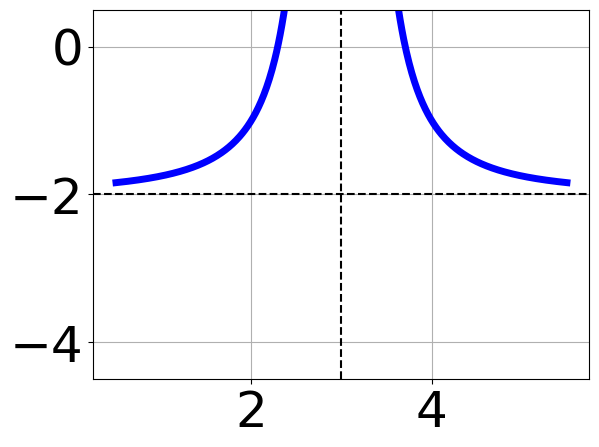
\includegraphics[width=0.3\textwidth]{../Figures/rationalEquationToGraphCopyCB.png}
\end{center}\begin{enumerate}[label=\Alph*.]
\begin{multicols}{2}
\item 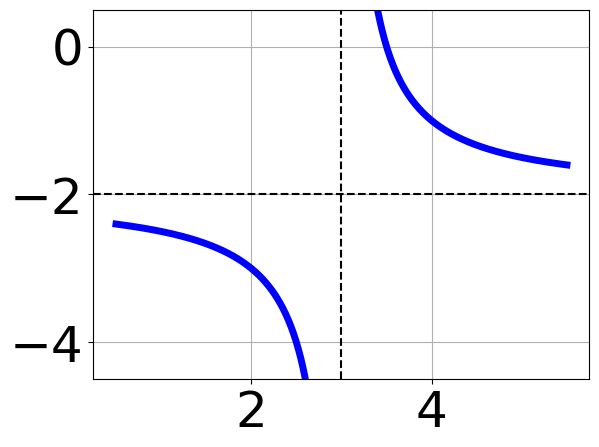
\includegraphics[width = 0.3\textwidth]{../Figures/rationalEquationToGraphCopyAB.png}
\item 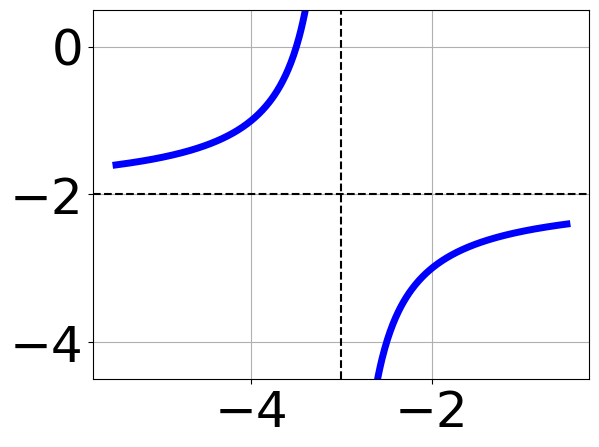
\includegraphics[width = 0.3\textwidth]{../Figures/rationalEquationToGraphCopyBB.png}
\item 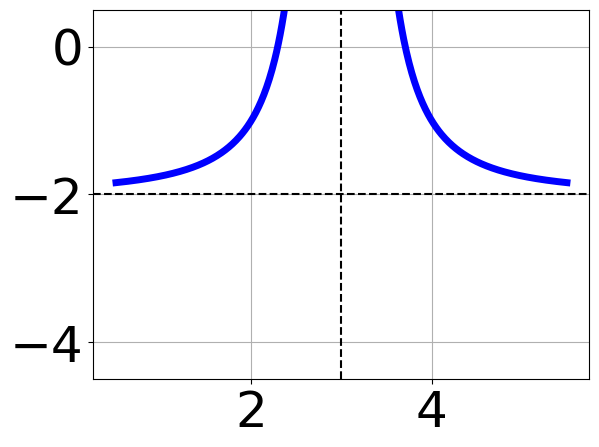
\includegraphics[width = 0.3\textwidth]{../Figures/rationalEquationToGraphCopyCB.png}
\item 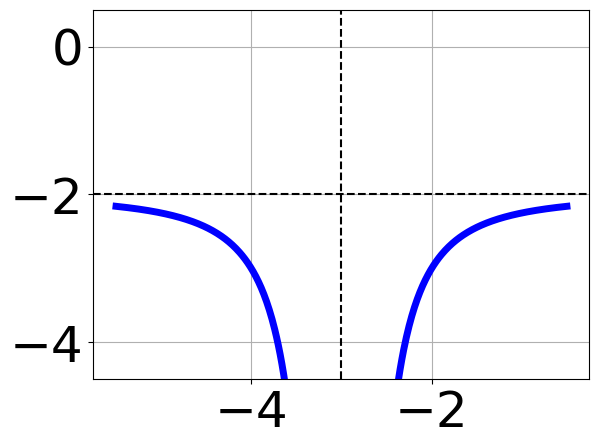
\includegraphics[width = 0.3\textwidth]{../Figures/rationalEquationToGraphCopyDB.png}
\end{multicols}\item None of the above.\end{enumerate}
\textbf{General Comment:} Remember that the general form of a basic rational equation is $ f(x) = \frac{a}{(x-h)^n} + k$, where $a$ is the leading coefficient (and in this case, we assume is either $1$ or $-1$), $n$ is the degree (in this case, either $1$ or $2$), and $(h, k)$ is the intersection of the asymptotes.
}
\litem{
Choose the graph of the equation below.
\[ f(x) = \frac{1}{(x - 3)^2} - 1 \]The solution is the graph below, which is option C.
\begin{center}
    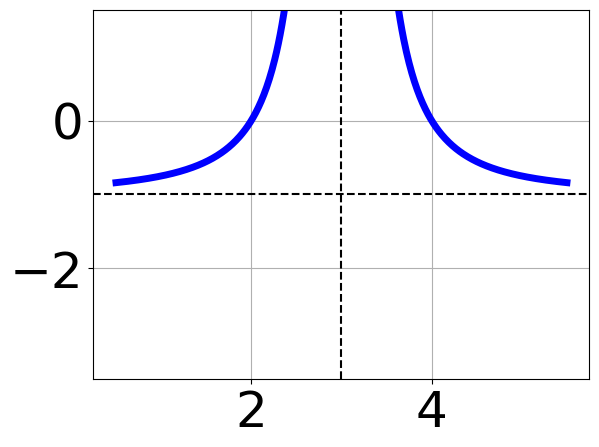
\includegraphics[width=0.3\textwidth]{../Figures/rationalEquationToGraphCB.png}
\end{center}\begin{enumerate}[label=\Alph*.]
\begin{multicols}{2}
\item 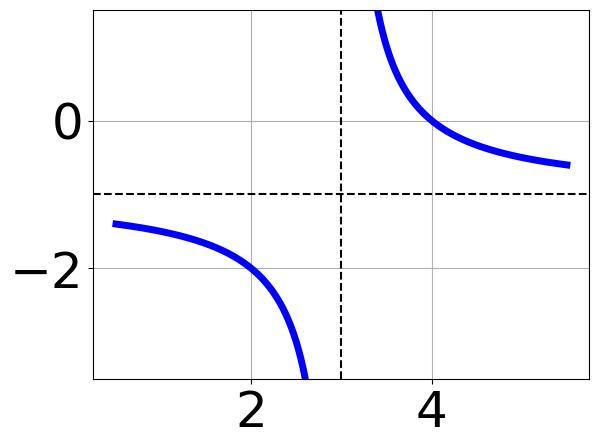
\includegraphics[width = 0.3\textwidth]{../Figures/rationalEquationToGraphAB.png}
\item 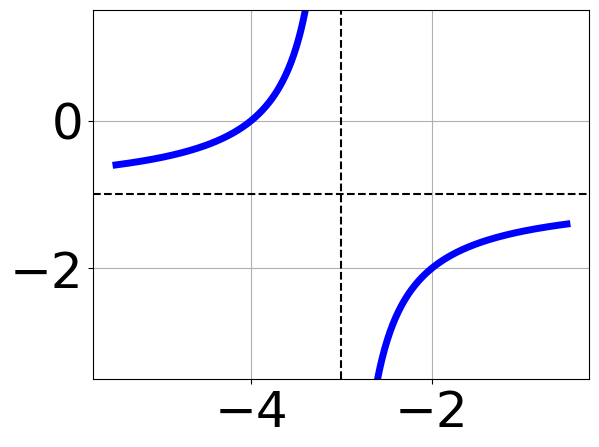
\includegraphics[width = 0.3\textwidth]{../Figures/rationalEquationToGraphBB.png}
\item 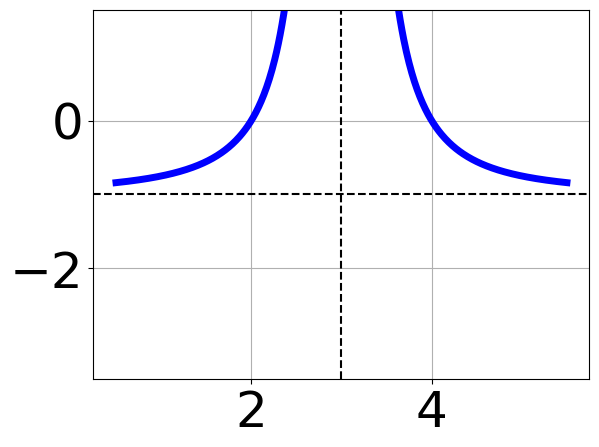
\includegraphics[width = 0.3\textwidth]{../Figures/rationalEquationToGraphCB.png}
\item 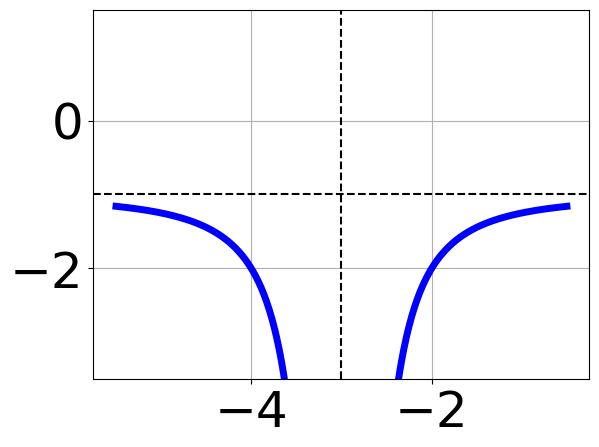
\includegraphics[width = 0.3\textwidth]{../Figures/rationalEquationToGraphDB.png}
\end{multicols}\item None of the above.\end{enumerate}
\textbf{General Comment:} Remember that the general form of a basic rational equation is $ f(x) = \frac{a}{(x-h)^n} + k$, where $a$ is the leading coefficient (and in this case, we assume is either $1$ or $-1$), $n$ is the degree (in this case, either $1$ or $2$), and $(h, k)$ is the intersection of the asymptotes.
}
\litem{
Choose the equation of the function graphed below.

\begin{center}
    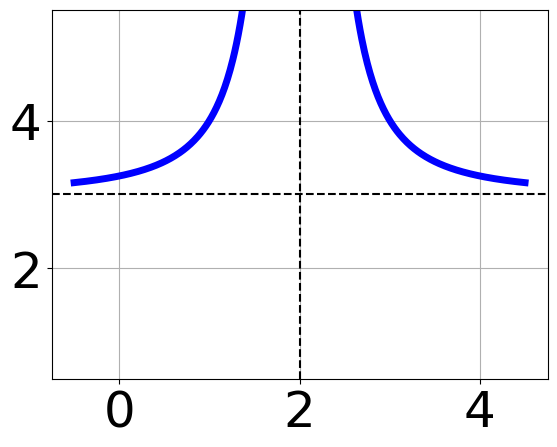
\includegraphics[width=0.5\textwidth]{../Figures/rationalGraphToEquationCopyB.png}
\end{center}


The solution is \( \text{None of the above as it should be } f(x) = \frac{1}{(x - 2)^2} + 3 \), which is option E.\begin{enumerate}[label=\Alph*.]
\item \( f(x) = \frac{-1}{x - 2} + 3 \)

Corresponds to thinking the graph was a shifted version of $\frac{1}{x}$, using the general form $f(x) = \frac{a}{(x-h)^2}+k$, and the opposite leading coefficient.
\item \( f(x) = \frac{1}{x + 2} + 3 \)

Corresponds to thinking the graph was a shifted version of $\frac{1}{x}$.
\item \( f(x) = \frac{-1}{(x - 2)^2} + 3 \)

Corresponds to using the general form $f(x) = \frac{a}{(x-h)^2}+k$ and the opposite leading coefficient.
\item \( f(x) = \frac{1}{(x + 2)^2} + 3 \)

The $x$-value of the equation does not match the graph.
\item \( \text{None of the above} \)

None of the equation options were the correct equation.
\end{enumerate}

\textbf{General Comment:} Remember that the general form of a basic rational equation is $ f(x) = \frac{a}{(x-h)^n} + k$, where $a$ is the leading coefficient (and in this case, we assume is either $1$ or $-1$), $n$ is the degree (in this case, either $1$ or $2$), and $(h, k)$ is the intersection of the asymptotes.
}
\litem{
Solve the rational equation below. Then, choose the interval(s) that the solution(s) belongs to.
\[ \frac{3x}{5x + 6} + \frac{-5x^{2}}{10x^{2} +22 x + 12} = \frac{-4}{2x + 2} \]The solution is \( \text{There are two solutions: } x = -25.042 \text{ and } x = -0.958 \), which is option B.\begin{enumerate}[label=\Alph*.]
\item \( x_1 \in [-25.06, -25.02] \text{ and } x_2 \in [-1.2,-1.19] \)


\item \( x_1 \in [-25.06, -25.02] \text{ and } x_2 \in [-1,-0.85] \)

* $x = -25.042 \text{ and } x = -0.958$, which is the correct option.
\item \( x \in [-1.02,-0.97] \)


\item \( x \in [-0.99,-0.93] \)


\item \( \text{All solutions lead to invalid or complex values in the equation.} \)


\end{enumerate}

\textbf{General Comment:} Distractors are different based on the number of solutions. Remember that after solving, we need to make sure our solution does not make the original equation divide by zero!
}
\litem{
Determine the domain of the function below.
\[ f(x) = \frac{4}{12x^{2} -36 x + 24} \]The solution is \( \text{All Real numbers except } x = 1.000 \text{ and } x = 2.000. \), which is option A.\begin{enumerate}[label=\Alph*.]
\item \( \text{All Real numbers except } x = a \text{ and } x = b, \text{ where } a \in [0.8, 1.4] \text{ and } b \in [1.7, 2.6] \)

All Real numbers except $x = 1.000$ and $x = 2.000$, which is the correct option.
\item \( \text{All Real numbers except } x = a, \text{ where } a \in [15.7, 17] \)

All Real numbers except $x = 16.000$, which corresponds to removing a distractor value from the denominator.
\item \( \text{All Real numbers.} \)

This corresponds to thinking the denominator has complex roots or that rational functions have a domain of all Real numbers.
\item \( \text{All Real numbers except } x = a \text{ and } x = b, \text{ where } a \in [15.7, 17] \text{ and } b \in [16.3, 19.5] \)

All Real numbers except $x = 16.000$ and $x = 18.000$, which corresponds to not factoring the denominator correctly.
\item \( \text{All Real numbers except } x = a, \text{ where } a \in [0.8, 1.4] \)

All Real numbers except $x = 1.000$, which corresponds to removing only 1 value from the denominator.
\end{enumerate}

\textbf{General Comment:} Recall that dividing by zero is not a real number. Therefore the domain is all real numbers \textbf{except} those that make the denominator 0.
}
\litem{
Choose the equation of the function graphed below.

\begin{center}
    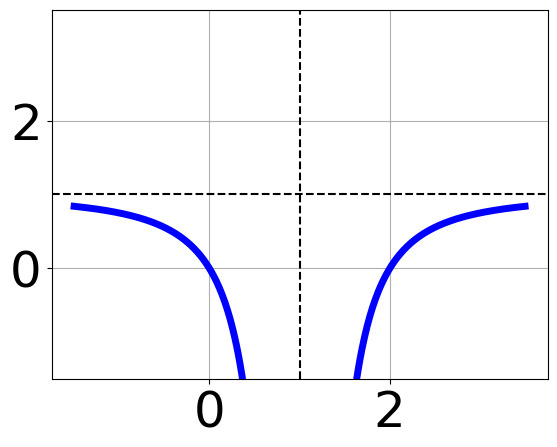
\includegraphics[width=0.5\textwidth]{../Figures/rationalGraphToEquationB.png}
\end{center}


The solution is \( f(x) = \frac{-1}{(x - 1)^2} + 1 \), which is option D.\begin{enumerate}[label=\Alph*.]
\item \( f(x) = \frac{1}{x + 1} + 1 \)

Corresponds to thinking the graph was a shifted version of $\frac{1}{x}$, using the general form $f(x) = \frac{a}{(x+h)^2}+k$, and the opposite leading coefficient.
\item \( f(x) = \frac{-1}{x - 1} + 1 \)

Corresponds to thinking the graph was a shifted version of $\frac{1}{x}$.
\item \( f(x) = \frac{1}{(x + 1)^2} + 1 \)

Corresponds to using the general form $f(x) = \frac{a}{(x+h)^2}+k$ and the opposite leading coefficient.
\item \( f(x) = \frac{-1}{(x - 1)^2} + 1 \)

This is the correct option.
\item \( \text{None of the above} \)

This corresponds to believing the vertex of the graph was not correct.
\end{enumerate}

\textbf{General Comment:} Remember that the general form of a basic rational equation is $ f(x) = \frac{a}{(x-h)^n} + k$, where $a$ is the leading coefficient (and in this case, we assume is either $1$ or $-1$), $n$ is the degree (in this case, either $1$ or $2$), and $(h, k)$ is the intersection of the asymptotes.
}
\litem{
Solve the rational equation below. Then, choose the interval(s) that the solution(s) belongs to.
\[ \frac{-3}{5x + 4} + 4 = \frac{-6}{15x + 12} \]The solution is \( x = -0.750 \), which is option E.\begin{enumerate}[label=\Alph*.]
\item \( x_1 \in [-0.85, -0.71] \text{ and } x_2 \in [0.85,2.85] \)

$x = -0.750 \text{ and } x = 0.850$, which corresponds to getting the correct solution and believing there should be a second solution to the equation.
\item \( \text{All solutions lead to invalid or complex values in the equation.} \)

This corresponds to thinking $x = -0.750$ leads to dividing by zero in the original equation, which it does not.
\item \( x \in [0.75,1.05] \)

$x = 0.850$, which corresponds to not distributing the factor $5x + 4$ correctly when trying to eliminate the fraction.
\item \( x_1 \in [-0.97, -0.78] \text{ and } x_2 \in [-1.75,0.25] \)

$x = -0.950 \text{ and } x = -0.750$, which corresponds to getting the correct solution and believing there should be a second solution to the equation.
\item \( x \in [-0.75,0.25] \)

* $x = -0.750$, which is the correct option.
\end{enumerate}

\textbf{General Comment:} Distractors are different based on the number of solutions. Remember that after solving, we need to make sure our solution does not make the original equation divide by zero!
}
\litem{
Solve the rational equation below. Then, choose the interval(s) that the solution(s) belongs to.
\[ \frac{18}{18x + 81} + 1 = \frac{18}{18x + 81} \]The solution is \( \text{all solutions are invalid or lead to complex values in the equation.} \), which is option E.\begin{enumerate}[label=\Alph*.]
\item \( x_1 \in [-5.5, -3.5] \text{ and } x_2 \in [-5.5,-3.5] \)

$x = -4.500 \text{ and } x = -4.500$, which corresponds to getting the correct solution and believing there should be a second solution to the equation.
\item \( x \in [-4.5,-2.5] \)

$x = -4.500$, which corresponds to not checking if this value leads to dividing by 0 in the original equation and thus is not a valid solution.
\item \( x \in [4.5,6.5] \)

$x = 4.500$, which corresponds to not distributing the factor $18x + 81$ correctly when trying to eliminate the fraction.
\item \( x_1 \in [-5.5, -3.5] \text{ and } x_2 \in [4.5,6.5] \)

$x = -4.500 \text{ and } x = 4.500$, which corresponds to getting the correct solution and believing there should be a second solution to the equation.
\item \( \text{All solutions lead to invalid or complex values in the equation.} \)

*$x = -4.500$ leads to dividing by 0 in the original equation and thus is not a valid solution, which is the correct option.
\end{enumerate}

\textbf{General Comment:} Distractors are different based on the number of solutions. Remember that after solving, we need to make sure our solution does not make the original equation divide by zero!
}
\end{enumerate}

\end{document}